\section{AND}

\subsection{Проверка того, находится ли значение на границе $2^n$}

Если нужно проверить, делится ли ваше значение на число вида 
$2^n$ (как 1024, 4096, итд.) без остатка,
вы можете использовать оператор \TT{\%} в \CCpp, но есть способ проще.
4096 это 0x1000, так что в нем всегда есть $4*3=12$ нулевых младших бит.

Что вам нужно, это просто:

\begin{lstlisting}[style=customc]
if (value&0xFFF)
{
	printf ("значение не делится на 0x1000 (или 4096)\n");
	printf ("кстати, остаток=%d\n", value&0xFFF);
}
else
	printf ("значение делится на 0x1000 (или 4096)\n");
\end{lstlisting}

Другими словами, это код проверяет, если здесь любой выставленный бит среди младших 12-и бит.
В качестве побочного эффекта, младщие 12 бит это всегда остаток от деления значения на 4096 (потому что деление на $2^n$
это лишь сдвиг вправо, и сдвинутые (или выброшенные) биты это биты остатка.

Та же история, если вам нужно проверить, является ли число четным или нет:

\begin{lstlisting}[style=customc]
if (value&1)
	// нечетное
else
	// четное
\end{lstlisting}

Это то же самое, как и деление на 2 и вычисление 1-битного остатка.

\subsection{Кирилличная кодировка KOI-8R}

Было время, когда 8-битная таблица \ac{ASCII} не поддерживалась некоторыми сервисами в Интернете, включая электронную почту.
Некоторые поддерживали, некоторые другие --- нет.

И это также было время, когда не-латинские системы письменности использовали вторую половину 8-битной таблицы ASCII
для размещения не-латинских символов.
Было несколько популярный кирилличных кодировок, но KOI-8R (придуманная Андреем ``ache'' Черновым)
в каком-то смысле уникальная, если сравнивать с другими.

% TODO invert arrow 
% TODO text latex form instead of png!
\begin{figure}[H]
\centering
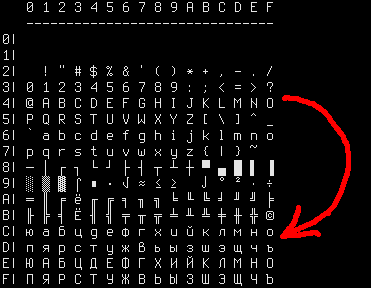
\includegraphics[width=0.5\textwidth]{fundamentals/koi8r.png}
\caption{KOI8-R table}
\end{figure}

Кое-кто может заметить, что кирилличные символы расположены почти в том же порядке, в котором и латинские.
Это приводит к важному свойству: если в кирилличном тексте закодированном в KOI-8R сбросить 8-й бит,
текст трансформируется в транслитерированный текст с латинскими символами на месте кирилличных.
Например, фраза на русском:

\begin{framed}
\begin{quotation}
Мой дядя самых честных правил, Когда не в шутку занемог, Он уважать себя заставил, И лучше выдумать не мог.
\end{quotation}
\end{framed}

\dots если закодирована в KOI-8R, и затем со сброшенным 8-м битом, трансформируется в:

\begin{framed}
\begin{quotation}
mOJ DQDQ SAMYH \^{}ESTNYH PRAWIL, kOGDA NE W [UTKU ZANEMOG, oN UWAVATX SEBQ ZASTAWIL, i LU\^{}[E WYDUMATX NE MOG.
\end{quotation}
\end{framed}

\dots конечно, выглядит это не очень эстетично, но этот текст читаем для тех, кто знает русский язык.

Следовательно, кирилличный текст закодированный в KOI-8R, пропущенный чере сервис поддерживающий только 7 бит,
выживет в виде транслитерированного, но читаемого текста.

Очистка 8-го бита автоматически транспонирует любой символ из второй половины (любой) 8-битной \ac{ASCII}-таблицы
в первую половину, в то же место (посмотрите на красную стрелку справа от таблицы).
Если символ уже расположен в первой половине (т.е., он находился в стандартной 7-битной \ac{ASCII}-таблице),
он не будет транспонироваться.

Вероятно, транслитерированный текст все еще можно восстановить, если вы прибавите 8-й бит к символам,
которые выглядят как транслитерированные.

Недостаток виден сразу: кирилличные символы расположенные в таблице KOI-8R расположены не в том порядке,
в каком они расположены в русском/болгарском/украинском/итд алфавите, и это не удобно для сортировки, например.

